%
%Не забыть:
%--------------------------------------
%Вставить колонтитулы, поменять название на титульнике



%--------------------------------------

\documentclass[a4paper, 12pt]{article} 

%--------------------------------------
%Russian-specific packages
%--------------------------------------
%\usepackage[warn]{mathtext}
\usepackage[T2A]{fontenc}
\usepackage[utf8]{inputenc}
\usepackage[english,russian]{babel}
\usepackage[intlimits]{amsmath}
\usepackage{esint}
%--------------------------------------
%Hyphenation rules
%--------------------------------------
\usepackage{hyphenat}
\hyphenation{ма-те-ма-ти-ка вос-ста-нав-ли-вать}
%--------------------------------------
%Packages
%--------------------------------------
\usepackage{amsmath}
\usepackage{amssymb}
\usepackage{amsfonts}
\usepackage{amsthm}
\usepackage{latexsym}
\usepackage{mathtools}
\usepackage{etoolbox}%Булевые операторы
\usepackage{extsizes}%Выставление произвольного шрифта в \documentclass
\usepackage{geometry}%Разметка листа
\usepackage{indentfirst}
\usepackage{wrapfig}%Создание обтекаемых текстом объектов
\usepackage{fancyhdr}%Создание колонтитулов
\usepackage{setspace}%Настройка интерлиньяжа
\usepackage{lastpage}%Вывод номера последней страницы в документе, \lastpage
\usepackage{soul}%Изменение параметров начертания
\usepackage{hyperref}%Две строчки с настройкой гиперссылок внутри получаеммого
\usepackage[usenames,dvipsnames,svgnames,table,rgb]{xcolor}% pdf-документа
\usepackage{multicol}%Позволяет писать текст в несколько колонок
\usepackage{cite}%Работа с библиографией
\usepackage{subfigure}% Человеческая вставка нескольких картинок
\usepackage{tikz}%Рисование рисунков
% Для картинок Моти
\usepackage{misccorr}
\usepackage{lscape}
\usepackage{cmap}


\usepackage{graphicx,xcolor}
\graphicspath{{Pictures/}}
\DeclareGraphicsExtensions{.pdf,.png,.jpg}

%----------------------------------------
%Список окружений
%----------------------------------------
\newenvironment {theor}[2]
{\smallskip \par \textbf{#1.} \textit{#2}  \par $\blacktriangleleft$}
{\flushright{$\blacktriangleright$} \medskip \par} %лемма/теорема с доказательством
\newenvironment {proofn}
{\par $\blacktriangleleft$}
{$\blacktriangleright$ \par} %доказательство
%----------------------------------------
%Список команд
%----------------------------------------
\newcommand{\grad}
{\mathop{\mathrm{grad}}\nolimits} %градиент

\newcommand{\diver}
{\mathop{\mathrm{div}}\nolimits} %дивергенция

\newcommand{\Def}[1]
{\underline{\textbf{#1}}} %определение

\newcommand{\RN}[1]
{\MakeUppercase{\romannumeral #1}} %римские цифры

\newcommand {\theornp}[2]
{\textbf{#1.} \textit{ #2} \par} %Написание леммы/теоремы без доказательства

\newcommand{\qrq}
{\ensuremath{\quad \Rightarrow \quad}} %Человеческий знак следствия

\newcommand{\qlrq}
{\ensuremath{\quad \Leftrightarrow \quad}} %Человеческий знак равносильности

\renewcommand{\phi}{\varphi} %Нормальный знак фи

\newcommand{\me}
{\ensuremath{\mathbb{E}}}

\newcommand{\md}
{\ensuremath{\mathbb{D}}}



%\renewcommand{\vec}{\overline}




%----------------------------------------
%Разметка листа
%----------------------------------------
\geometry{top = 3cm}
\geometry{bottom = 2cm}
\geometry{left = 1.5cm}
\geometry{right = 1.5cm}
%----------------------------------------
%Колонтитулы
%----------------------------------------
\pagestyle{fancy}%Создание колонтитулов
\fancyhead{}
%\fancyfoot{}
\fancyhead[R]{\textsc{Резонанс в RLC цепях}}%Вставить колонтитул сюда
%----------------------------------------
%Интерлиньяж (расстояния между строчками)
%----------------------------------------
%\onehalfspacing -- интерлиньяж 1.5
%\doublespacing -- интерлиньяж 2
%----------------------------------------
%Настройка гиперссылок
%----------------------------------------
\hypersetup{				% Гиперссылки
	unicode=true,           % русские буквы в раздела PDF
	pdftitle={Заголовок},   % Заголовок
	pdfauthor={Автор},      % Автор
	pdfsubject={Тема},      % Тема
	pdfcreator={Создатель}, % Создатель
	pdfproducer={Производитель}, % Производитель
	pdfkeywords={keyword1} {key2} {key3}, % Ключевые слова
	colorlinks=true,       	% false: ссылки в рамках; true: цветные ссылки
	linkcolor=blue,          % внутренние ссылки
	citecolor=blue,        % на библиографию
	filecolor=magenta,      % на файлы
	urlcolor=cyan           % на URL
}
%----------------------------------------
%Работа с библиографией (как бич)
%----------------------------------------
\renewcommand{\refname}{Список литературы}%Изменение названия списка литературы для article
%\renewcommand{\bibname}{Список литературы}%Изменение названия списка литературы для book и report
%----------------------------------------
\begin{document}
	\begin{titlepage}
		\begin{center}
			$$$$
			$$$$
			$$$$
			$$$$
			{\Large{НАЦИОНАЛЬНЫЙ ИССЛЕДОВАТЕЛЬСКИЙ УНИВЕРСИТЕТ}}\\
			\vspace{0.1cm}
			{\Large{ВЫСШАЯ ШКОЛА ЭКОНОМИКИ}}\\
			\vspace{0.25cm}
			{\large{Факультет физики}}\\
			\vspace{5.5cm}
			{\Huge\textbf{{Лабораторная работа}}}\\%Общее название
			\vspace{1cm}
			{\LARGE{<<Резонанс в RLC цепях>>}}\\%Точное название
			\vspace{2cm}
			{Работу выполнил студент 2 курса}\\
			{Захаров Сергей Дмитриевич}
			\vfill
			
\includegraphics[width = 0.2\textwidth]{HSElogo}\\
			\vfill
			Москва\\
			2019
		\end{center}
	\end{titlepage}

\tableofcontents

\newpage

\section{Цели работы}

Перед выполнением работы были поставлены следующие цели:

\begin{enumerate}
	\item Построить резонансную кривую для последовательного и параллельного RLC контуров.
	
	\item Экспериментально определить с ее помощью частоту резонанса.
	
	\item Определить добротность контуров.
	
	\item Для параллельного соединения построить зависимость разности фаз от частоты источника.
\end{enumerate}

\section{Описание метода выполнения работы}

В целом, теоретические выкладки в данной лабораторной работе особенно не требуется. Отметим лишь, что теоретическую частоту резонанса с целью ее дальнейшего сравнения с реальной можно посчитать следующим образом:

\begin{equation}
	\omega_{res} = \frac{1}{\sqrt{L \cdot C}}
	\label{eq:omegath}
\end{equation}

Кроме того, чтобы найти добротность, мы найдем отношение резонансной частоты к ширине резонансной кривой на высоте $\dfrac{1}{\sqrt{2}}$ от максимальной:

\begin{equation}
	Q = \frac{w_{res}}{\Delta \omega}
	\label{eq:Q}
\end{equation}

\section{Выполнение работы}

\subsection{Последовательное соединение}

Для проведения работы были взяты элементы со следующими параметрами:

\begin{itemize}
	\item $R = 98.54 \pm 0.01$ кОм
	
	\item $C = 86.9 \pm 0.1$ мкФ
	
	\item $L = 514.2 \pm 0.1$ мкГн
\end{itemize}


Первым делом была собрана схема, представленная на рисунке \ref{fig:series}.

\begin{figure}[h!]
	\centering
	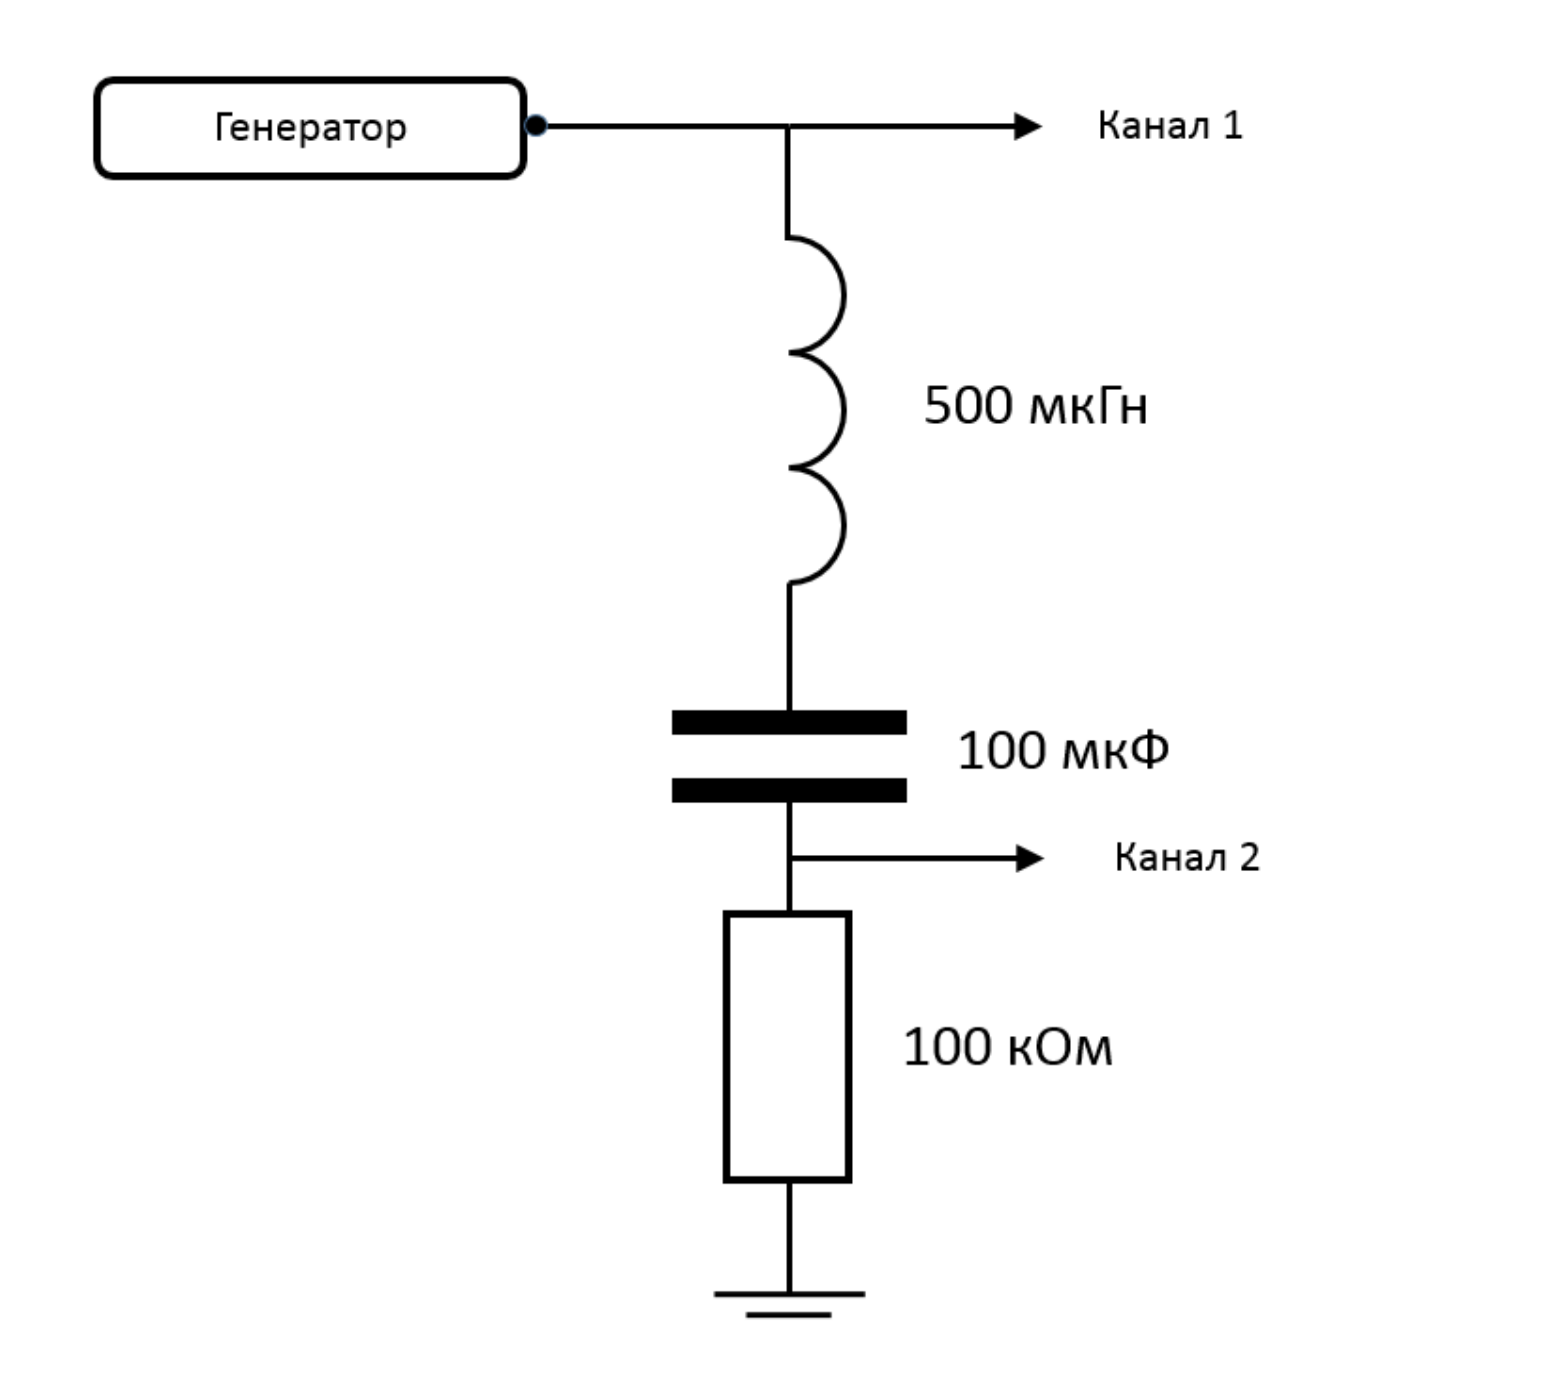
\includegraphics[width=0.4\linewidth]{Series}
	\caption{Схема последовательной RLC цепи}
	\label{fig:series}
\end{figure}

Затем была произведена серия измерений амплитуд колебаний напряжения на сопротивлении при одной и той же амплитуде генератора (10 В), но при различных его частотах. Полученная кривая и является искомой резонансной кривой, она представлена на рисунке \ref{fig:resonance_curve}.

\begin{figure}[h!]
	\centering
	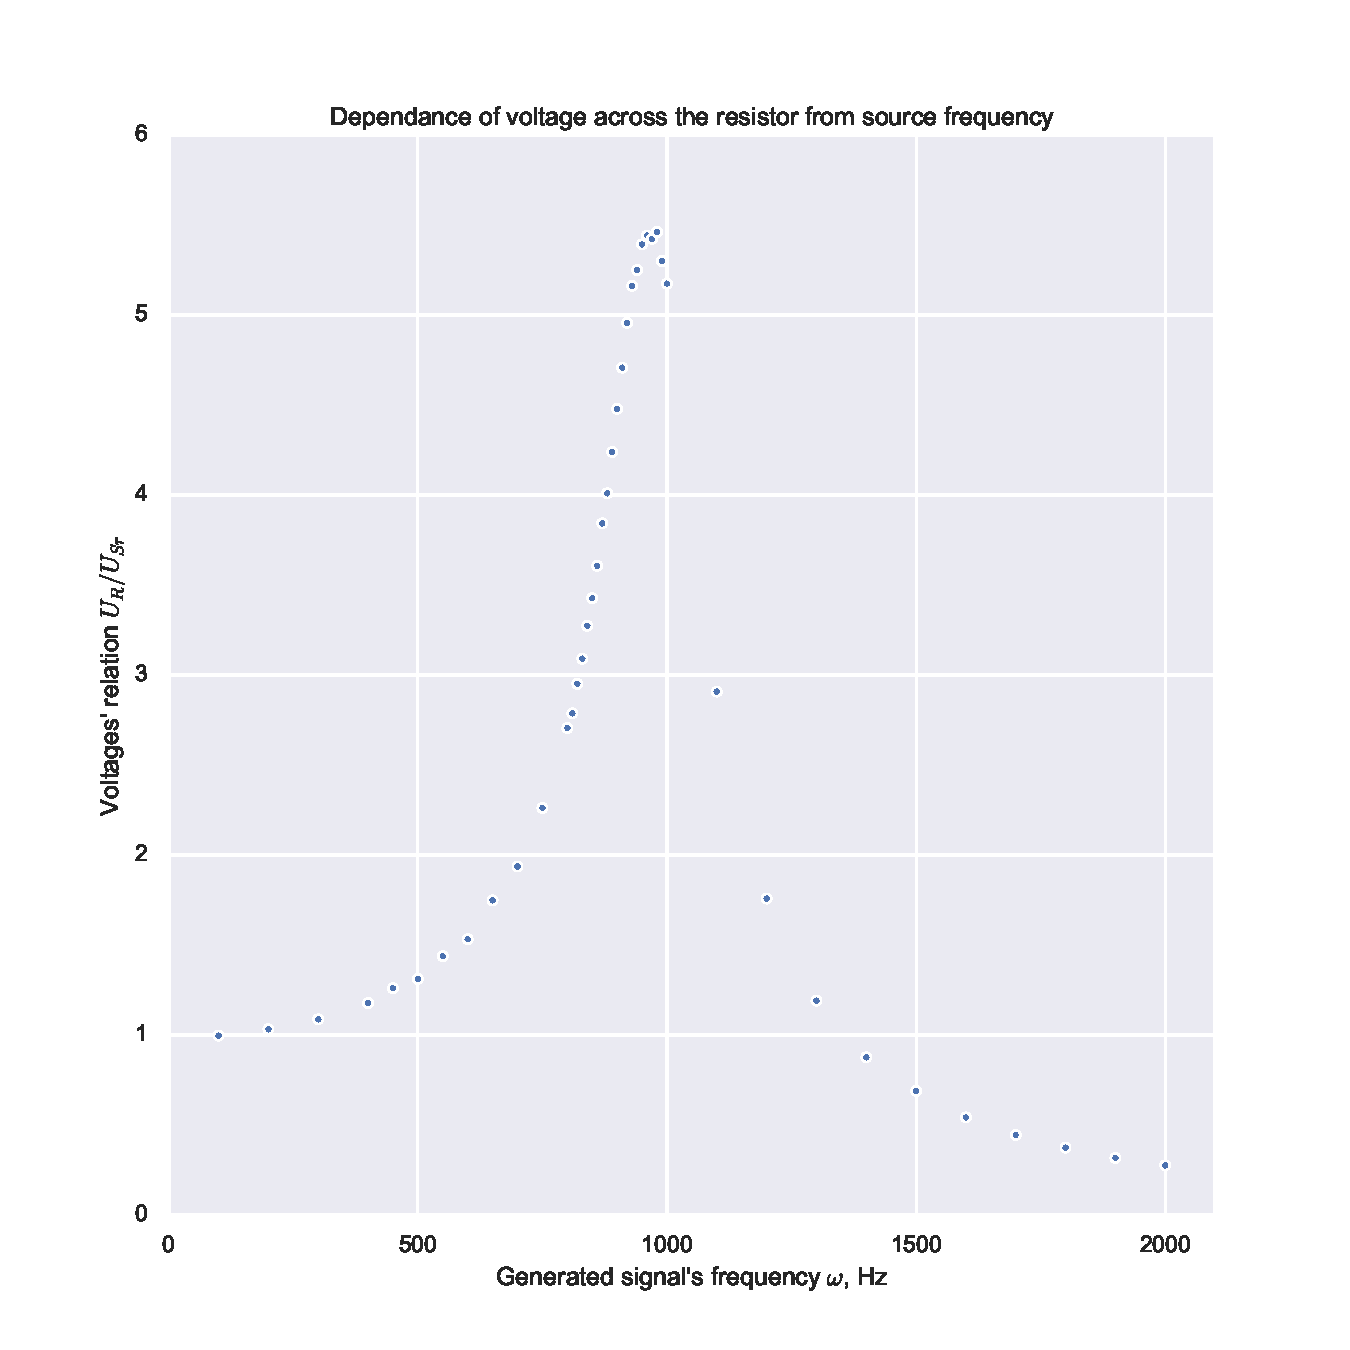
\includegraphics[width=0.7\linewidth]{Series_connection}
	\caption{Резонансная кривая для последовательной RLC цепи}
	\label{fig:resonance_curve}
\end{figure}

На основании полученных данных становится возможным получить экспериментальную добротность с помощью ($\ref{eq:Q}$). Она оказывается равной $\boxed{Q = 3.2}$.


Кроме того, возможно также определить и реальную резонансную частоту. Она оказывается равна $\boxed{\omega_{real} = 6157 \text{ кГц}}$

Ради интереса сравним ее с теоретической частотой, которую можно посчитать по формуле~$\ref{eq:omegath}$: $\boxed{w_{th} = 4.7 \text{ кГц}}$

Отметим, что полученные величины сильно отличаются, на целых 3 порядка. Это непорядок, надо понять, почему. Ответ оказывается достаточно простым: емкость конденсатора сильно падает с ростом частоты колебаний. Это было видно даже тогда, когда мы пытались измерить емкость конденсатора: при различных частотах, которые нам были доступны, достигались совершенно разные емкости. Это упомянуто, например, в \cite{Picture_source}. В качестве иллюстрации приведем картинку, представленную там, на рисунке $\ref{fig:imp}$.

\begin{figure}[h!]
	\centering
	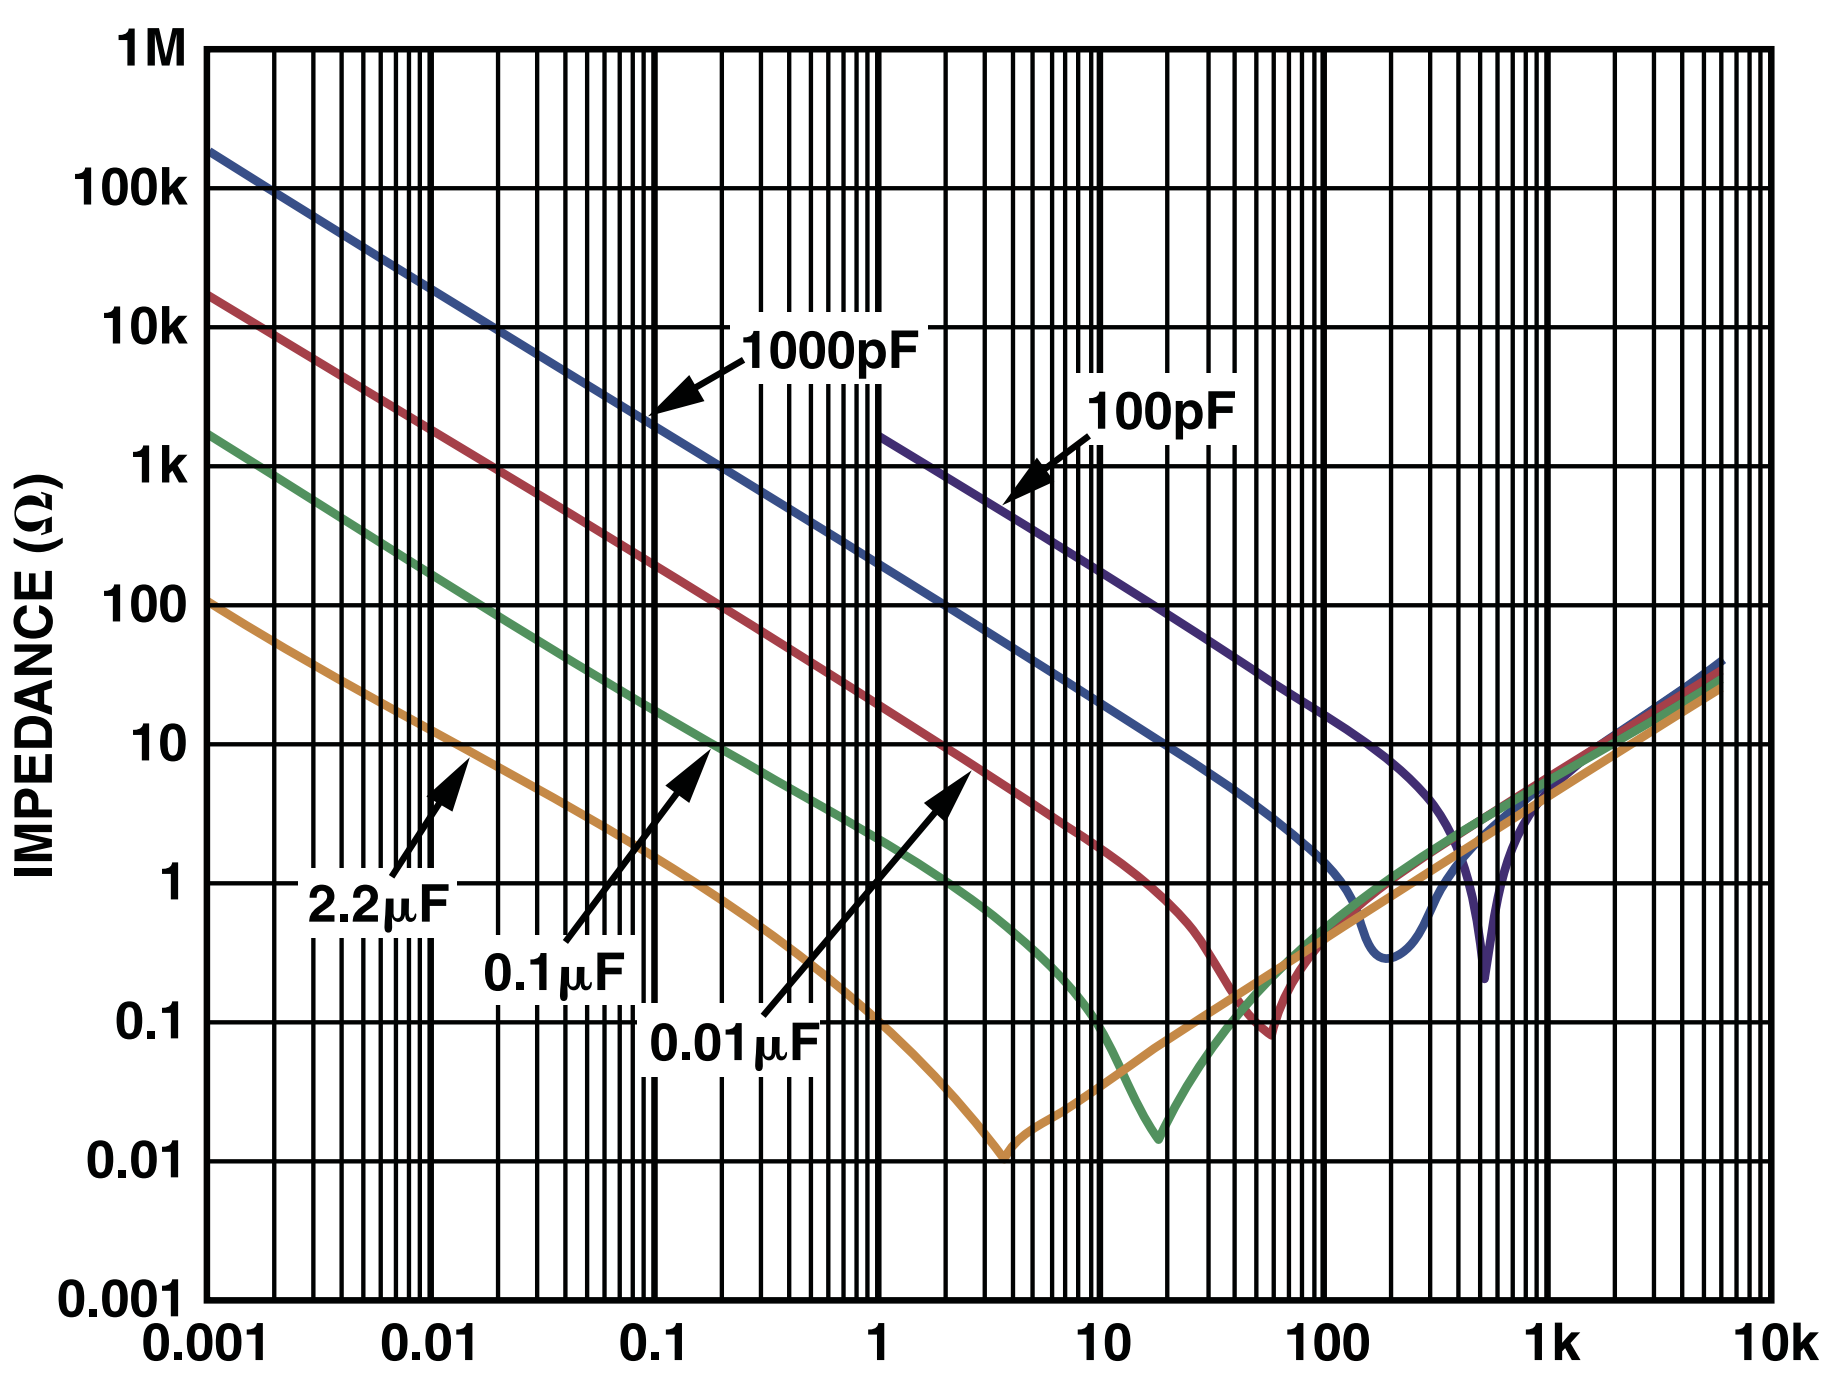
\includegraphics[width=0.8\textwidth]{Graphic}
	\caption{Зависимость импеданса конденсатора от частоты колебаний в контуре}
	\label{fig:imp}
\end{figure}

\subsection{Параллельное соединение}

Для проведения работы были взяты элементы со следующими параметрами:

\begin{itemize}
	\item $L = 514.2 \pm 0.1$ мкГн
	
	\item $C = 6.21$ нФ
	
	\item $R_1 = 1.01$ Ом
	
	\item $R_2 = 10.04$ кОм
\end{itemize}

Схема эксперимента представлена на рисунке \ref{fig:parallel}. На основании

\begin{figure}[h!]
	\centering
	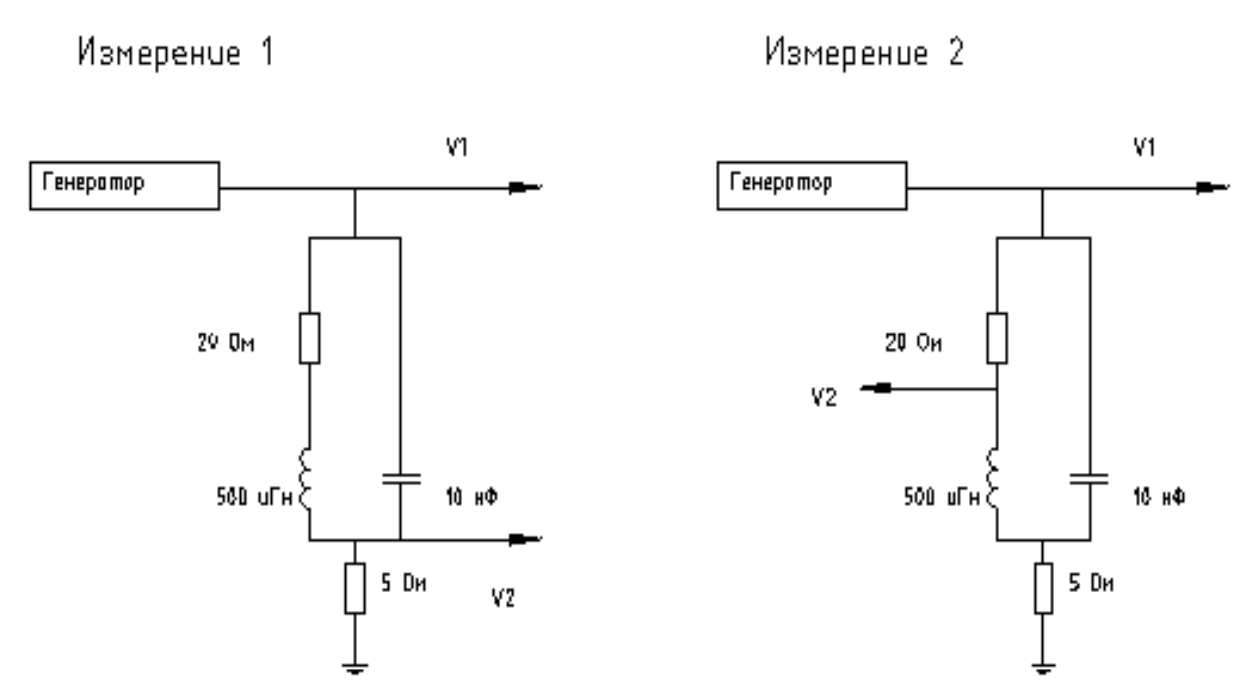
\includegraphics[width=0.7\textwidth]{Scheme_parallel}
	\caption{Схема параллельной RLC цепи}
	\label{fig:parallel}
\end{figure}

В ходе измерений была получена резонансная кривая, представленная на рисунке

\begin{figure}[h!]
	\centering
	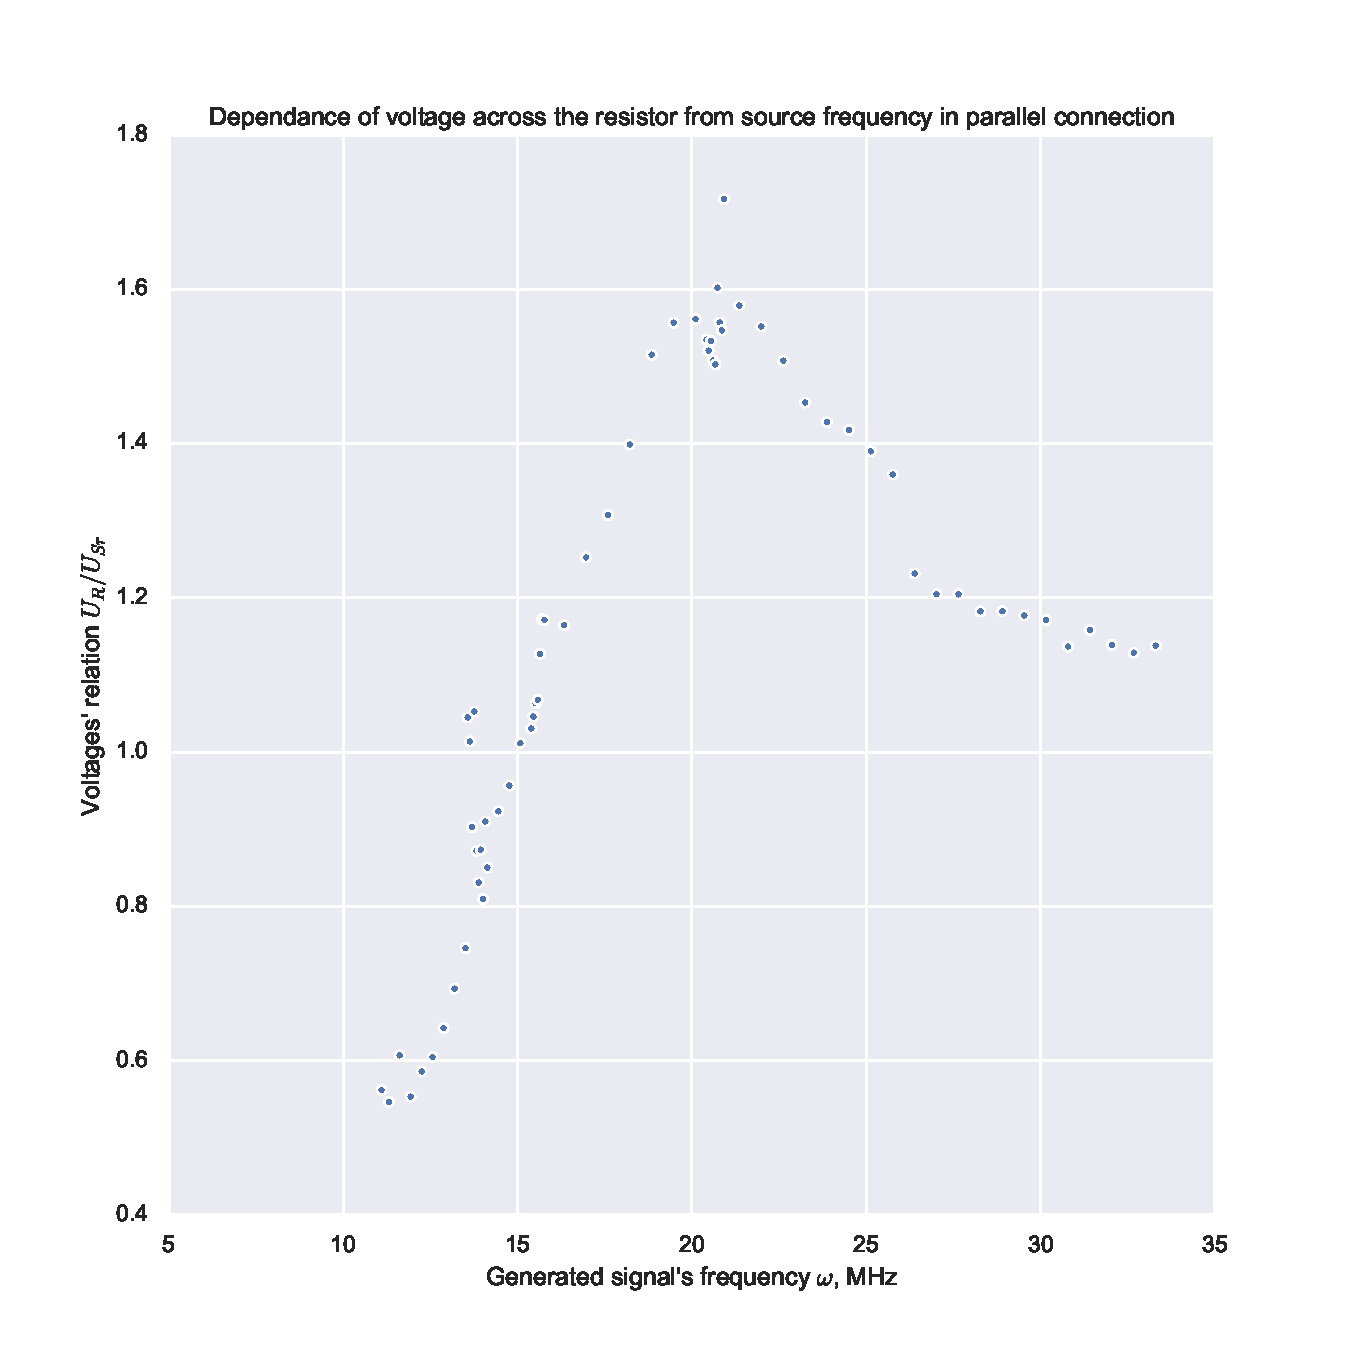
\includegraphics[width=\textwidth]{Parallel}
\end{figure}

Видно, что полученная картина нашим представлениям о резонансе не соответствует. По этой причине считать добротность не считаю необходимым.

Максимальным отношение амплитуда становится при частоте, которую мы с большой натяжкой можем назвать резонансной, при $\boxed{\omega_{rl} = 20 \text{ МГц}}$. Теоретическая же частота оказалась равной $\boxed{\omega_{th} = 32 \text{ кГц}}$. 

Еще одним интересным графиком является зависимость разности фаз от частоты источника, которая вобьет последний гвоздь в наши надежды о наличии в полученных данных резонанса. Она представлена на рисунке \ref{fig:phi}. Как видно, в столь желанный ноль она так и не обращается.

\begin{figure}[h!]
	\centering
	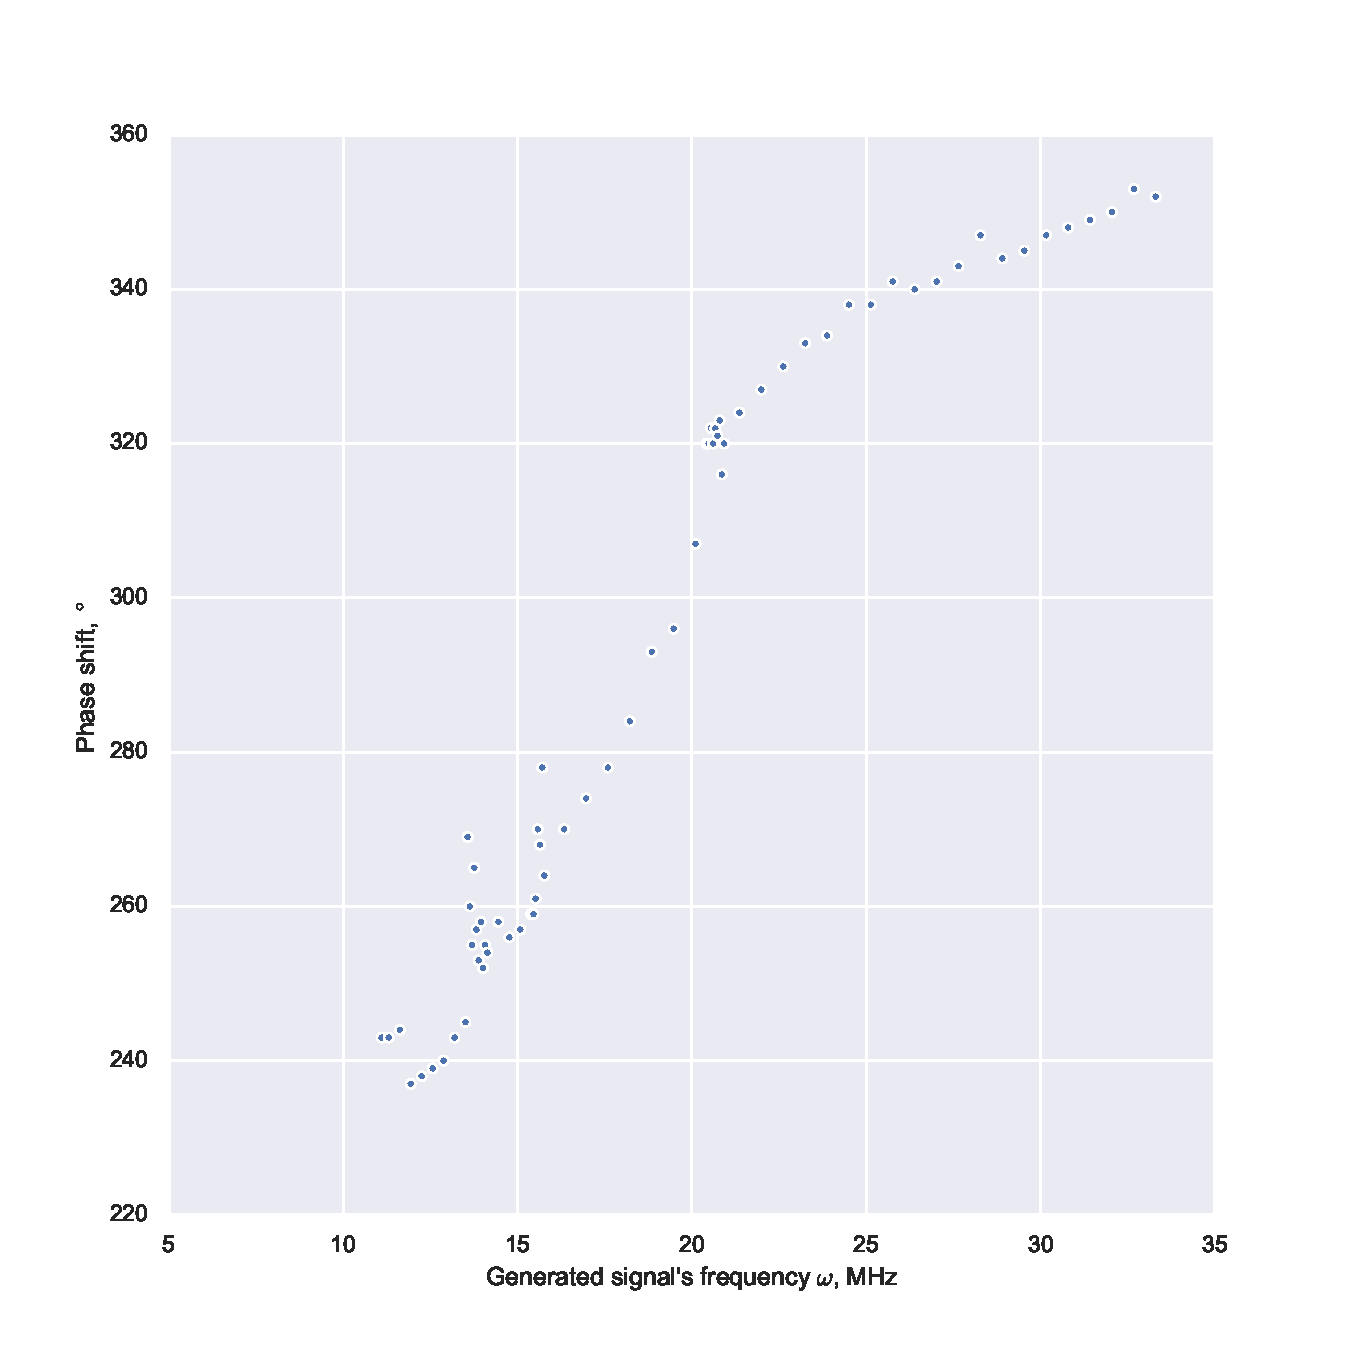
\includegraphics[width=\textwidth]{PhaseParallel}
	\caption{Зависимость разности фаз от частоты колебаний источника}
	\label{fig:phi}
\end{figure}

\section{Итоги}

В последовательной цепи резонанс все же удалось пронаблюдать, хоть и совершенно не на ожидаемой частоте. Связано это с тем, что емкость конденсатора сильно зависит от частоты колебаний контура.

В параллельной цепи же резонанс пронаблюдать не удалось в силу того, что генератор осциллографа не мог вытянуть необходимый сигнал.





\begin{thebibliography}{9}
	\addcontentsline{toc}{section}{\refname}
	\bibitem{Picture_source} John Ardizzoni. A Practical Guide to High-Speed Printed-Circuit-Board Layout
\end{thebibliography}




\end{document}





















